\section{Ejercicio 2}
\subsection{Descripcion}
El ejercio 2 consiste en realizar con CUFFT y FFFTW una FFT de real a complejos y la inversa,
y comprobar que ambas son inversas entre si (es decir, devuelven los valores originales).
Se utilizaron la libreria Thrust y CUFFT para las versiones en C++ de CPU y de GPU.

El ejercicio planteando incluia una funcion $f$ que es aplicada a un arreglo en la memoria de la GPU que contiene
una secuencia de $N$ numeros, fijado $N=1048576=2^{20}$. Este numero es bueno porque al ser m\'ultiplo de 2,
CUFFT reserva una cantidad exacta de m\'emoria, y no tiene que paddear ni redondear, ayudando a la performance 
\'optima de las funciones.

\subsection{TODOs}

El c\'odigo ya escrito en el enunciado realizaba una FFT de real a complejos a un arreglo del 0 a N al que se
le aplicaba una funci\'on $f$. La tarea que realizamos nosotros fue la de obtener la inversa de este valor.
Para eso, aplicamos las funciones definidas en la API de CUFFT, pero que deshagan las transformaciones.

Es decir, si la ida fue armada como 
\begin{itemize}
    \item Armar plan R2C para N elementos
    \item Disponer de un vector en la placa/en memoria para N/2+1 elementos para guardar resultado
    \item Correr el plan R2C con CUFFT/FFTW
\end{itemize}

La vuelta se va a armar como

\begin{itemize}
    \item Armar plan C2R para N elementos
    \item Disponer de un vector en la placa/en memoria para N elementos para guardar resultado
    \item Correr el plan C2R con CUFFT/FFTW
\end{itemize}


El detalle m\'as importante de esto fue darnos cuenta como recuperar los valores originales. Parece que es trivial
ya que vamos y volvemos con las ejecuciones de los planes, pero hay un comentario corto que esta en el manual de CUDA y de 
FFTW. Este dice que FFTW / CUFFT no normalizan, por lo que eso lo tiene que hacer uno. Es decir, cuando imprimimos
los valores originales para comprobar la exactitud de la ida y vuelta de la FFT, tenemos que reescalar el valor
final haciendo una division por la cantidad de elementos en el arreglo. Cuando nos percatamos de eso, fue trivial
la comparacion entre el dato de input y el de output.

Un detalle tambien importante para poder comparar en el caso de FFTW fue darnos cuenta que el plan \texttt{C2R} 
\textbf{no} preserva el input por default. Esto trajo dolores de cabeza a la hora de visualizar que los 
datos esten de la manera correcta. Se resuelve agregando el flag \texttt{FFTW\_PRESERVE\_INPUT} a la creaci\'on
del plan.

\subsection{Resultados}

%%%%%%%%%%%%%%%%%%%%%%%%%%%%%%%%%%%%%%%%%%%%%%%%%%%%%%%%%%%%%%%%
  \begin{figure}[H]
 \begin {center}
 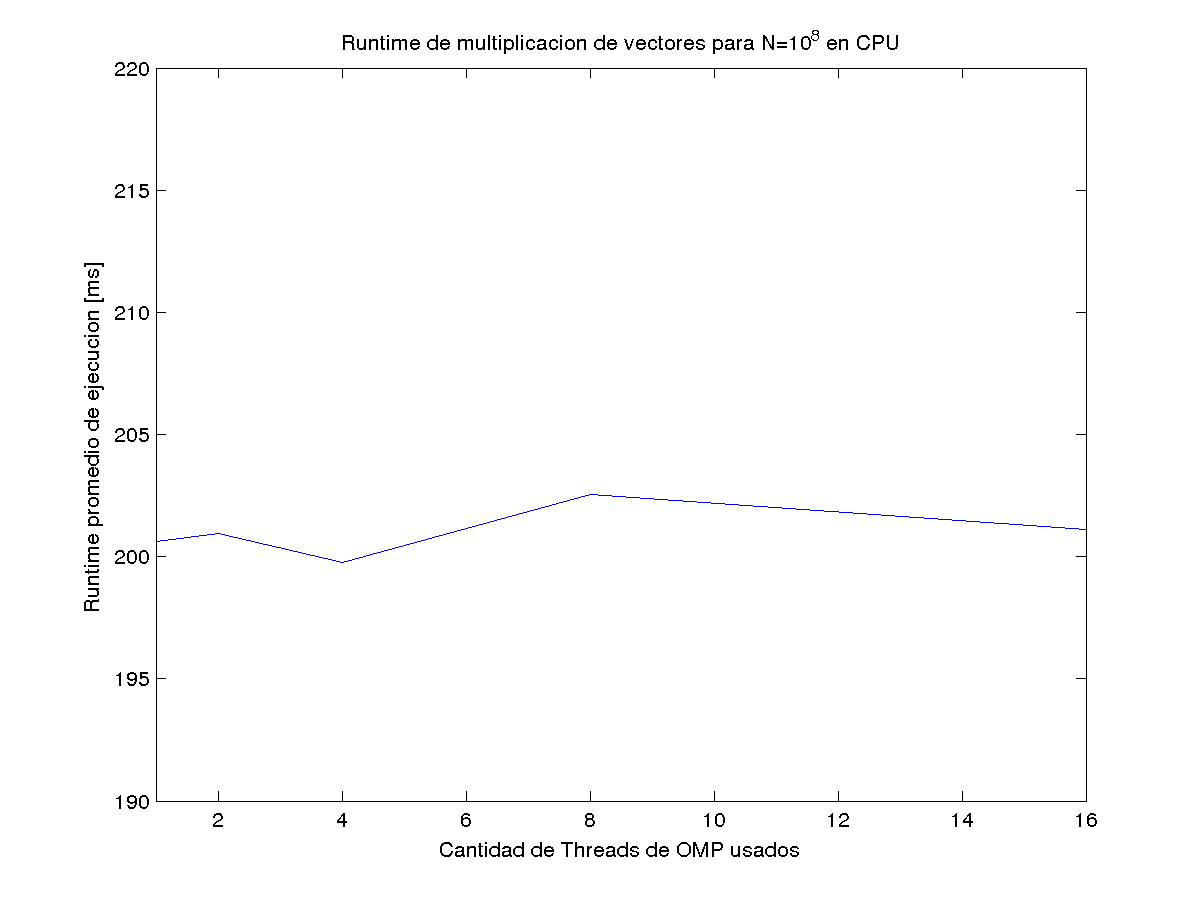
\includegraphics[width=\hrwidth]{plots/ej1omp.png}
 \end {center}
 \caption{Runtime del ej2 en Thrust con OMP, en funcion de la cantidad de threads, para una longitud de vectores $L=10^8$}
 \label{fig:ej1OMP}
 \end{figure}

\begin{table}
    \begin{tabular}{l|r|r}
        \textbf{M\'etodo} & \textbf{ Runtime Real 2 Complex [ms] } & \textbf{  Runtime Complex 2 Real [ms] } \\ \hline
        1 OMP Thread         & 200.598     & \\
        2 OMP Thread          & 200.963      &\\
        4 OMP Thread          & 199.766      &\\
        8 OMP Thread  & 202.534      &      \\
        16 OMP Thread & 201.127      &  \\
        CUDA M2090 & 11.035          &
    \end{tabular}
\end{table}

Los resultados muestran claramente que el calculo de FFT es un problema que paraleliza muy bien. En efecto,
es de crucial interes esto porque este algoritmo aparece en muchisimas ramas de la ciencia. Podemos apreciar
tambien que la libreria CUFFT es notablemente buena, siendo varias veces m\'as eficiente que las versiones
de CPU. 
